\section{Experimentación}

%Imagen 1
\begin{wrapfigure}{r}{0.6\textwidth}
  \vspace{-20pt}
  \begin{center}
    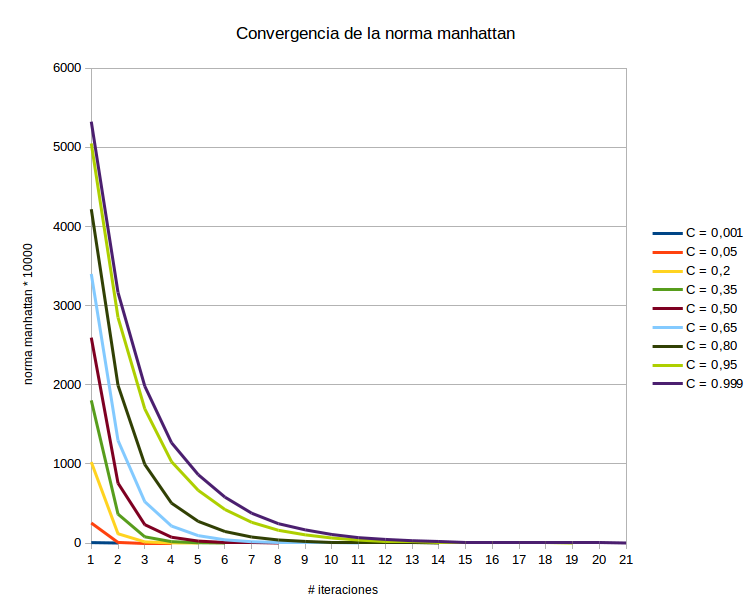
\includegraphics[scale= 0.6]{imagenes/convergencia1.png}
  \end{center}
  \vspace{-20pt}
   \caption{Con tantas páginas y tantos links.}
  \vspace{-10pt}
  \label{fig:img1}
\end{wrapfigure}

Para poder analizar la convergencia de PageRank realizamos mediciones de la cantidad de iteraciones que realiza el método de la potencia para el algoritmo, que termina cuando la norma de Manhattan es menor que un determinado valor muy cercano a 0.\\

Usamos tres instancias generadas al azar: La primera de 1000 páginas y 3000 links, la segunda de la misma cantidad de páginas pero 10000 links y la tercera de 500 páginas y 150000 links.\\

Nos interesa ver qué hace que el algoritmo termine en una menor cantidad de pasos y qué relación hay entre ese número y el valor de $c$. Ejecutamos $PageRank$ para cada instancia con una tolerancia fija de 0,00001, variando el valor del $c$ desde 0,001 hasta 0,999. Cada gráfico corresponde a los resultados obtenidos para una instancia distinta.\\



%Imagen 2
\begin{figure}[h]
  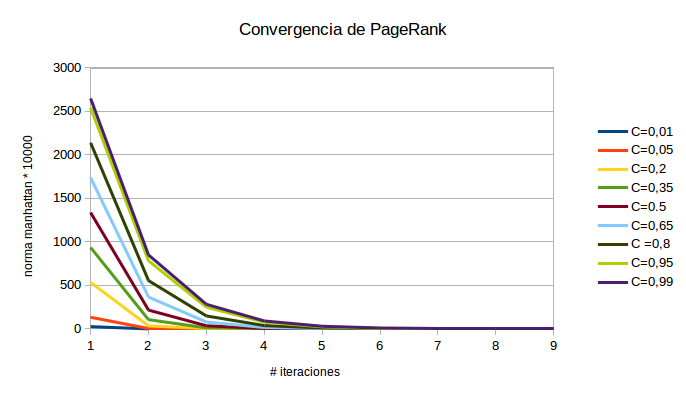
\includegraphics[scale= 0.6]{imagenes/convergencia2.png}
   \caption{Con tantas páginas y tantos links.}
  \label{fig:img1}
\end{figure}


\newpage

%Imagen 3
\begin{wrapfigure}{r}{0.6\textwidth}
  \vspace{-20pt}
  \begin{center}
    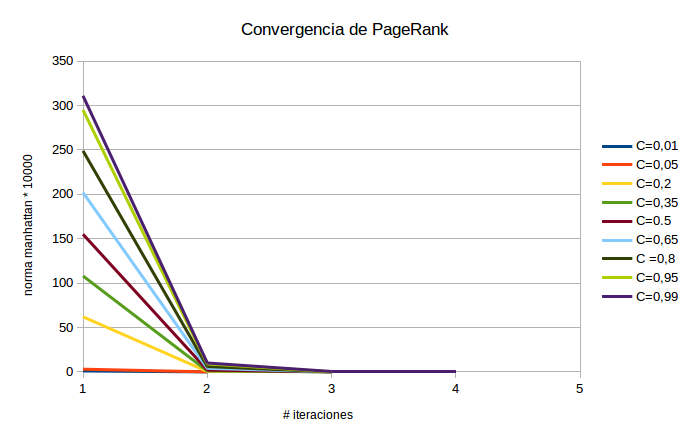
\includegraphics[scale= 0.6]{imagenes/convergencia3.png}
  \end{center}
  \vspace{-20pt}
   \caption{Con tantas páginas y tantos links.}
  \vspace{-10pt}
  \label{fig:img1}
\end{wrapfigure}

Mirando cada gráfico por separado podemos ver que la cantidad de iteraciones del algoritmo disminuye mientras más chico sea el valor de $c$, independientemente de que tan esparsa sea la matriz de links. 
Si comparamos los tres gráficos, vemos que las normas son mas chicas y el algoritmo converge más rápidamente mientras mas completa (menos esparsa) sea la matriz de links.\\



%% FALTA ANALISIS DE POR QUE PASA ESTO %%

%%%%%%%%%%%%%%%%%%%%%%%%%%%%%%%%%%%%%%%%%%%%%%%%%%%%%%%%%%%%%%%%%%%%%%%%%%%%%%%%%%%%%


Para ver como se comporta el algoritmo de $PageRank$ y comparar los resultados con los de $IN-DEG$, proponemos los siguientes ejemplos pequeños. Los grafos representan las páginas web y los link entre ellas, y las tablas muestran los resultados obtenidos de cada algoritmo.\\

%% ACA VAN LAS 6 IMAGENES DE GRAFOS , cada una junto a la tabla de resultados %%

%% ACA EL ANALISIS DE LOS RESULTADOS %%


